\chapter{Experimentation (Rooshan Khan)}
\label{Chapter4}
\lhead{Chapter 4. \emph{Experimentation}} % Write in your own chapter title to set the page header

\section{Phase 1}
Phase 1 of our project focused on fine-tuning BERT for the sentiment analysis task using the SST-5 and CFIMDB datasets. This phase aimed to understand the process of fine-tuning for a single task. We experimented with two fine-tuning strategies: (i) fine-tuning only the last linear layer, and (ii) fine-tuning the entire model. The development accuracies for both datasets under each strategy are presented in Table~\ref{tab:phase1_results}.
\begin{table}[H]
\centering
\caption{Quantitative Result of Phase 1. Accuracy comparison of BERT on SST and CFIMDB.}
\label{tab:phase1_results}
\begin{tabular}{l|cc|cc}
\toprule
 & \multicolumn{4}{c}{\textbf{Dev Accuracies}} \\
\midrule
 & \multicolumn{2}{c|}{\textbf{Ours}} & \multicolumn{2}{c}{\textbf{Reference}} \\
 & \textbf{SST} & \textbf{CFIMDB} & \textbf{SST} & \textbf{CFIMDB} \\
\midrule
last linear layer finetuning & 0.409 & 0.788 & 0.390 & 0.780 \\
full model finetuning        & 0.524 & 0.967 & 0.515 & 0.966 \\
\bottomrule
\end{tabular}
\end{table}

\section{Phase 2}
Imagine that we need separate models for different tasks. The biggest issue in this case is memory consumption. Storing 110 million parameters for each model becomes highly inefficient—n tasks would require n separate models, resulting in a total of 110n million parameters.

Why not use the same BERT model for all tasks? The question is: how? One approach is to share the 12 BERT layers across all tasks while using separate task-specific heads. This idea is illustrated in Figure~\ref{fig:Proposed Model}.
\begin{figure}[H]
    \centering
    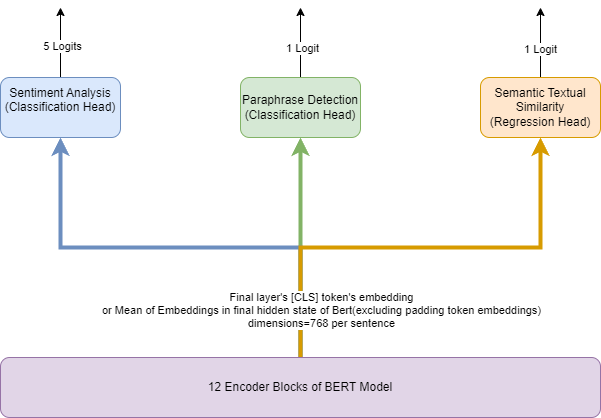
\includegraphics[width=0.8\linewidth]{Figures/Proposed_Model.png}
    \caption{Proposed Model}
    \label{fig:Proposed Model}
\end{figure}

We used Colab's L4 GPU for training and evaluating our models. Initially, we adopted a \texttt{batch\_size=32}, which worked well for baseline training. However, the introduction of SMART regularization significantly increased memory usage, leading to CUDA out-of-memory (OOM) errors.

For the Sentiment Analysis task, we were able to apply SMART successfully with \texttt{batch\_size=32} without encountering memory issues. However, for the Semantic Textual Similarity (STS) task, training with SMART triggered CUDA OOM errors, prompting us to lower the batch size to \texttt{16}.

Later, during training for the Paraphrase Detection task, we found that even \texttt{batch\_size=16} caused CUDA OOM errors. As a result, we further reduced the batch size to \texttt{8} for this task to ensure successful training.

The Architecture that we will be using throughout our experimentation is given in Figure~\ref{fig:Final_Model_Architecture}

\begin{figure}[H]
    \centering
    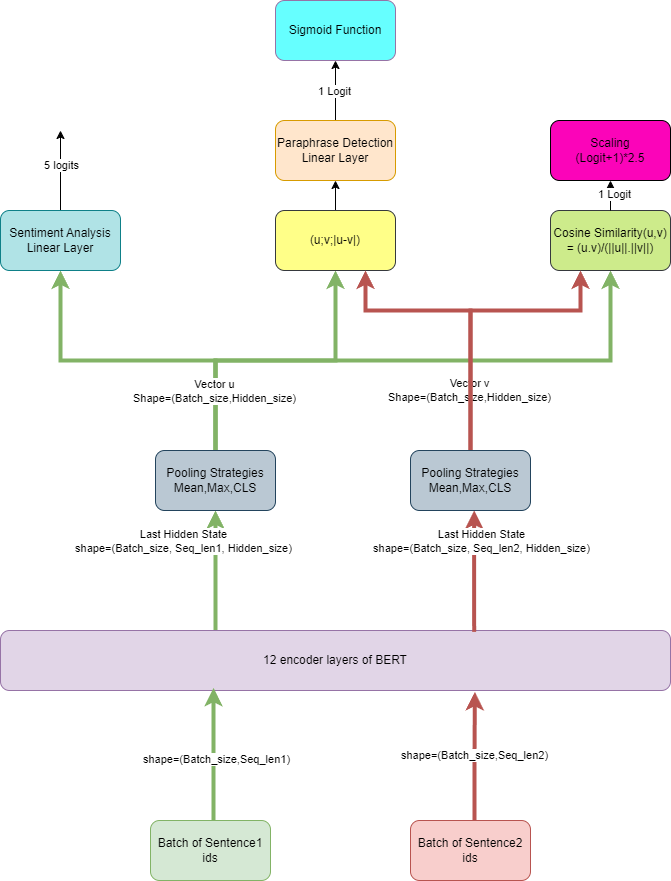
\includegraphics[width=0.8\linewidth]{Figures/Final Model Architecture.png}
    \caption{Final Model Architecture}
    \label{fig:Final_Model_Architecture}
\end{figure}


\subsection{Individually fine-tuned BERT models}
\label{subsec:Individually fine-tuned BERT models}
We first trained and tested our models on individual tasks. The best accuracy on the SST dataset was achieved using the mean of all vectors from the last hidden state corresponding to the input words (excluding padding tokens). We employed the SMART algorithm for training. The highest accuracy obtained was \textbf{0.533} at \textbf{epoch 7}. We set the hyperparameters as follows: \(\lambda_s = 10\) and \(\mu = 1\). A dropout rate of 0.3 was used during training. Look at Figure~\ref{fig:sst_accuracy}.
\begin{figure}[H]
    \centering
    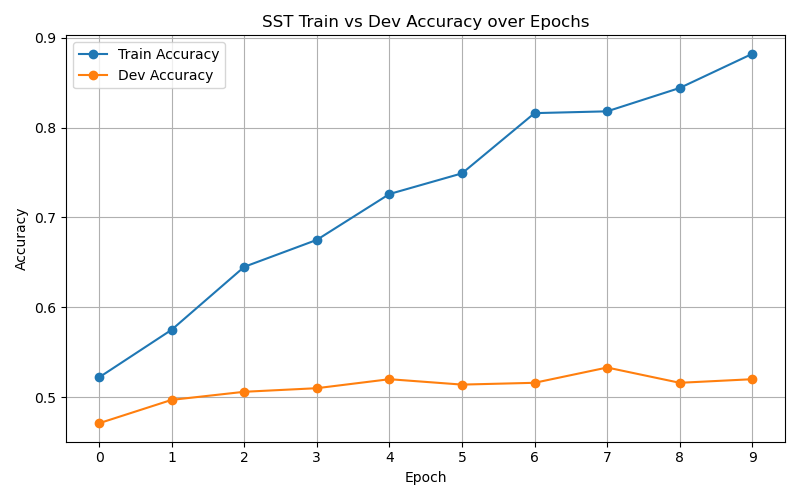
\includegraphics[width=0.8\linewidth]{Figures/sst_accuracy_plot.png}
    \caption{SST train vs dev accuracy over 10 epochs}
    \label{fig:sst_accuracy}
\end{figure}

When we trained our model on the Semantic Textual Similarity (STS) task alone, we achieved a best Pearson correlation of 0.821 on the development set. We achieved Pearson correlation on the first epoch. We used SBERT architecture with mean pooling for regression tasks that finds cosine similarity between sentences. We shifted and scaled this cosine similarity to be in the range from 0 to 5 instead of -1 to 1. We also used the SMART algorithm during training. We used $\lambda_s=5$ and $\mu=1$. A dropout rate of 0.3 was used during training. As shown in Figure~\ref{fig:sts_corr}, the dev STS correlation starts to drop after epoch 0, indicating potential overfitting.

\begin{figure}[H]
    \centering
    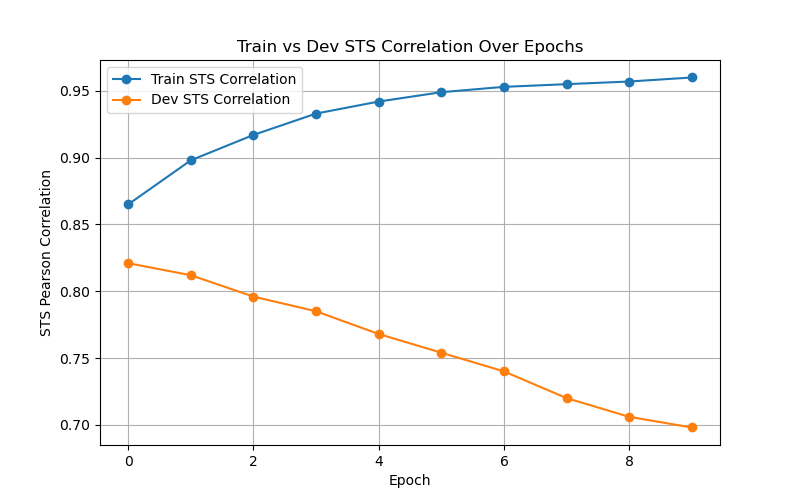
\includegraphics[width=0.8\linewidth]{Figures/sts_corr_plot.png}
    \caption{STS train vs dev correlation over 10 epochs}
    \label{fig:sts_corr}
\end{figure}

For the Paraphrase Detection task, our model achieved a maximum accuracy of 0.875 with hyperparameters set to $\lambda_s = 5$ and $\mu = 1$. Due to computational constraints, we trained the model for only one epoch. Specifically, incorporating SMART significantly increased training time to approximately 5 hours per epoch, which was not feasible given our limited compute resources. A dropout rate of 0.1 was used during training. Batch size was set to 8 to avoid CUDA out-of-memory error.  We used SBERT architecture with mean pooling for this classification task.

The results for separate models trained individually for each task are summarized in Table~\ref{tab:smart_per_task}.

\begin{table}[H]
    \centering
    \begin{tabular}{|l|l|c|}
    \hline
    \textbf{Task} & \textbf{Metric} & \textbf{Value} \\ 
    \hline
    Sentiment Classification (SST-5) & Accuracy & 0.533 \\ 
    \hline
    Paraphrase Detection (QQP) & Accuracy & 0.875 \\ 
    \hline
    Semantic Textual Similarity (STS-B) & Pearson Correlation & 0.821 \\ 
    \hline
    \end{tabular}
    \caption{Best performance of separate models fine-tuned individually for each task}
    \label{tab:smart_per_task}
\end{table}


% \begin{table}[h]
%     \centering
%     \caption{Performance with SMART Fine-Tuning Applied Independently per Task}
%     \label{tab:smart_per_task}
%     \begin{tabular}{|l|c|}
%     \hline
%     \textbf{Task} & \textbf{Best Metric Value} \\
%     \hline
%     Sentiment Classification (SST-5) Accuracy & 0.533 \\
%     Paraphrase Detection (QQP) Accuracy & 0.875 \\
%     Semantic Textual Similarity (STS-B) Pearson Correlation & 0.821 \\
%     \hline
%     \end{tabular}
% \end{table}

\subsection{Accuracies and Pearson Correlation for Fine-Tuning the same model on Multiple Tasks}
\subsubsection{Sequential Fine-Tuning: SBERT Only}

We trained the model for \textbf{3} epochs on the Paraphrase Detection task, \textbf{10} epochs on the Semantic Textual Similarity (STS) task, and \textbf{10} epochs on the Sentiment Analysis task.

\begin{table}[H]
    \centering
    \begin{tabular}{|l|l|c|}
    \hline
    \textbf{Task} & \textbf{Metric} & \textbf{Value} \\ \hline
    Paraphrase Detection & Accuracy & 0.6285 \\ \hline
    Semantic Textual Similarity (STS) & Pearson Correlation & 0.5444 \\ \hline
    Sentiment Analysis (SST) & Accuracy & 0.1698 \\ \hline
    \end{tabular}
    \caption{Development set performance before fine-tuning}
    \label{tab:pre_finetuning_metrics}
\end{table}

After training for 3 epochs on the QQP dataset, the best Paraphrase Detection accuracy achieved was \textbf{0.7441}. See Figure~\ref{fig:paraphrase_acc_plot} for the training and development curves.

\begin{figure}[H]
    \centering
    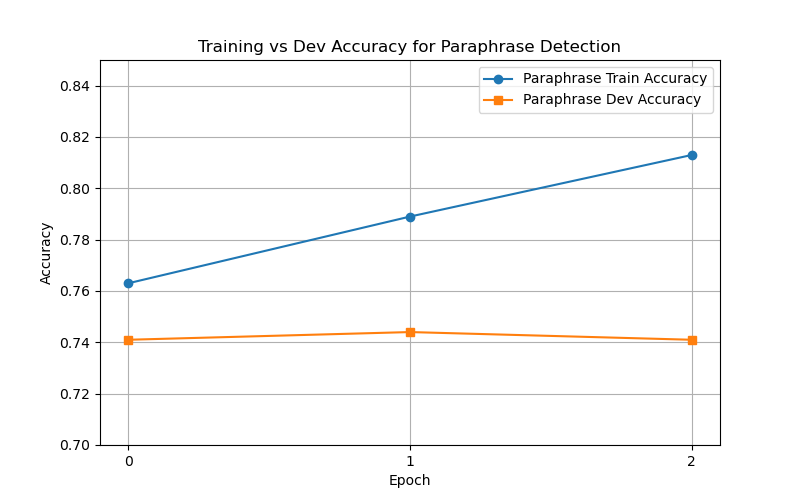
\includegraphics[width=0.8\textwidth]{Figures/Paraphrase_plot_3epochs_SBERT_Only.png}
    \caption{Train vs Dev Accuracy for Paraphrase Detection using SBERT Only (3 epochs)}
    \label{fig:paraphrase_acc_plot}
\end{figure}

\begin{table}[H]
    \centering
    \begin{tabular}{|l|l|c|}
    \hline
    \textbf{Task} & \textbf{Metric} & \textbf{Value} \\ \hline
    Paraphrase Detection & Accuracy & 0.7441 \\ \hline
    Semantic Textual Similarity (STS) & Pearson Correlation & 0.7127 \\ \hline
    Sentiment Analysis (SST) & Accuracy & 0.1735 \\ \hline
    \end{tabular}
    \caption{Development set performance after fine-tuning on Paraphrase Detection for 3 epochs}
    \label{tab:post_finetuning_paraphrase_metrics}
\end{table}

Subsequently, we fine-tuned the best-performing model for \textbf{10} epochs on the STS task.

\begin{figure}[H]
    \centering
    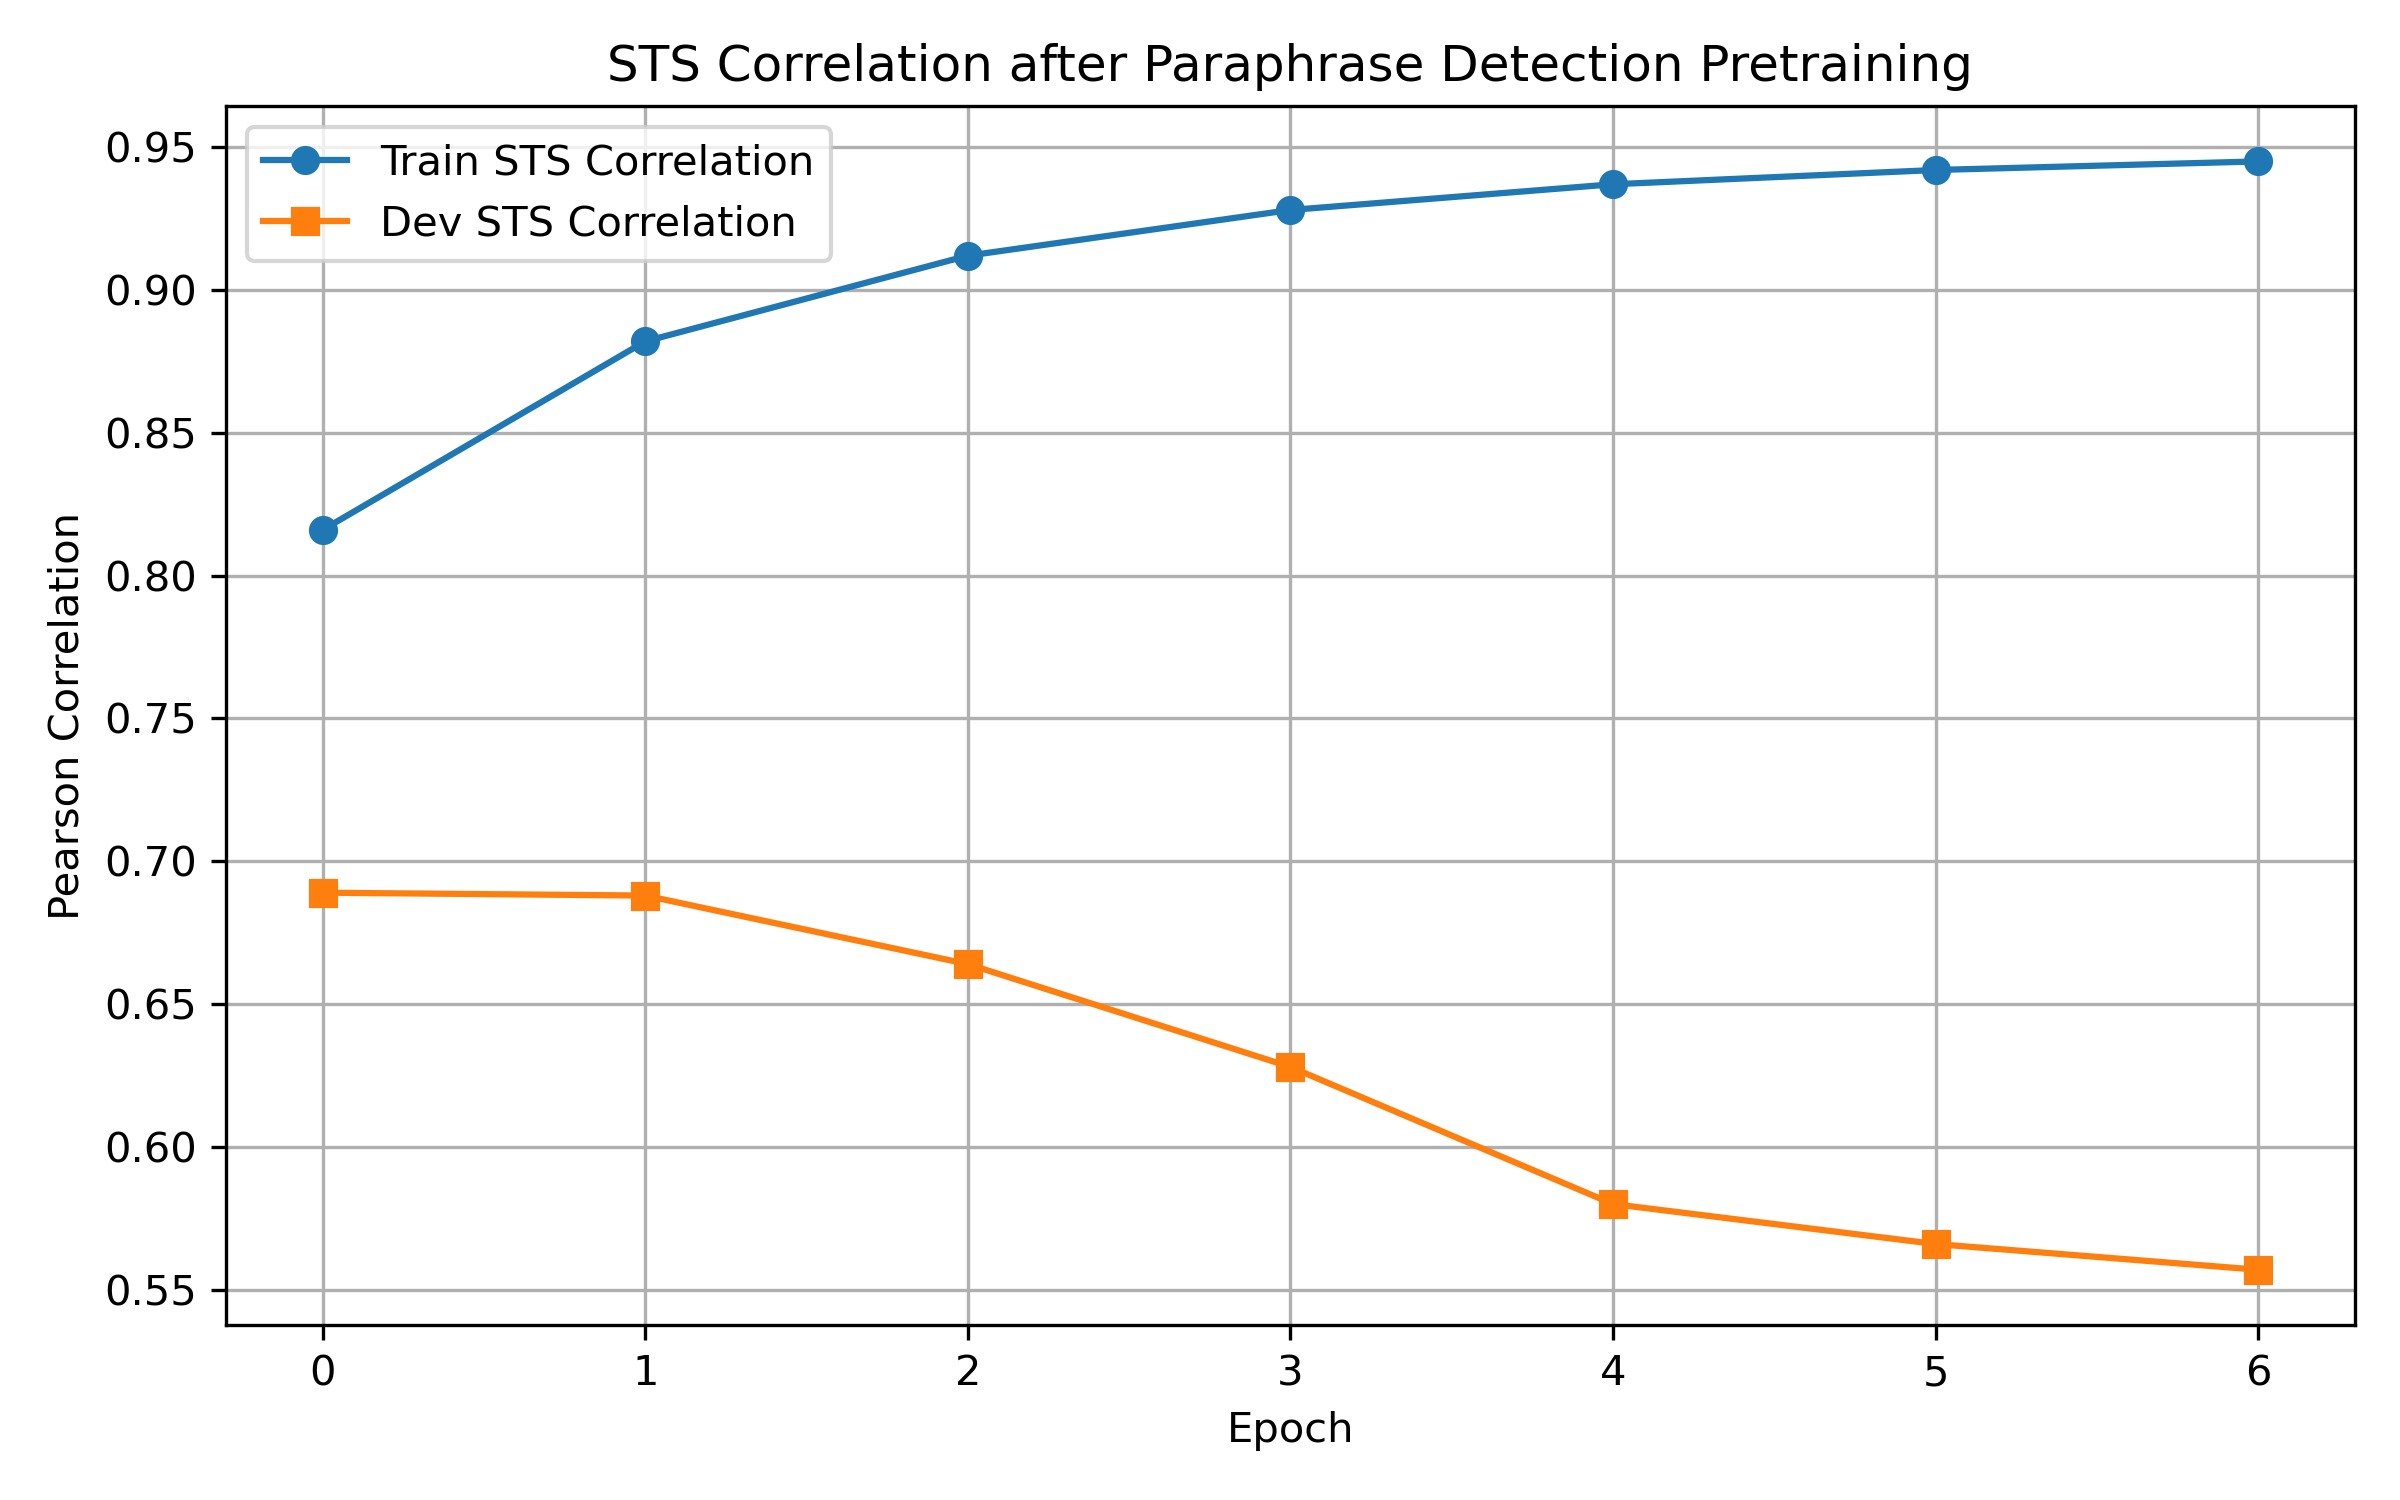
\includegraphics[width=0.6\textwidth]{Figures/STS_plot_10epochs_SBERT_Only.png}
    \caption{Train vs Dev Correlation for Semantic Textual Similarity using SBERT Only (10 epochs)}
    \label{fig:sts_corr_plot}
\end{figure}

\begin{table}[H]
    \centering
    \begin{tabular}{|l|l|c|}
    \hline
    \textbf{Task} & \textbf{Metric} & \textbf{Value} \\ \hline
    Paraphrase Detection & Accuracy & 0.8353 \\ \hline
    Semantic Textual Similarity (STS) & Pearson Correlation & 0.6890 \\ \hline
    Sentiment Analysis (SST) & Accuracy & 0.1835 \\ \hline
    \end{tabular}
    \caption{Development set performance after fine-tuning on the STS task}
    \label{tab:post_finetuning_sts_metrics}
\end{table}

Finally, we fine-tuned the best-performing model for \textbf{10} epochs on the Sentiment Analysis task.

\begin{figure}[H]
    \centering
    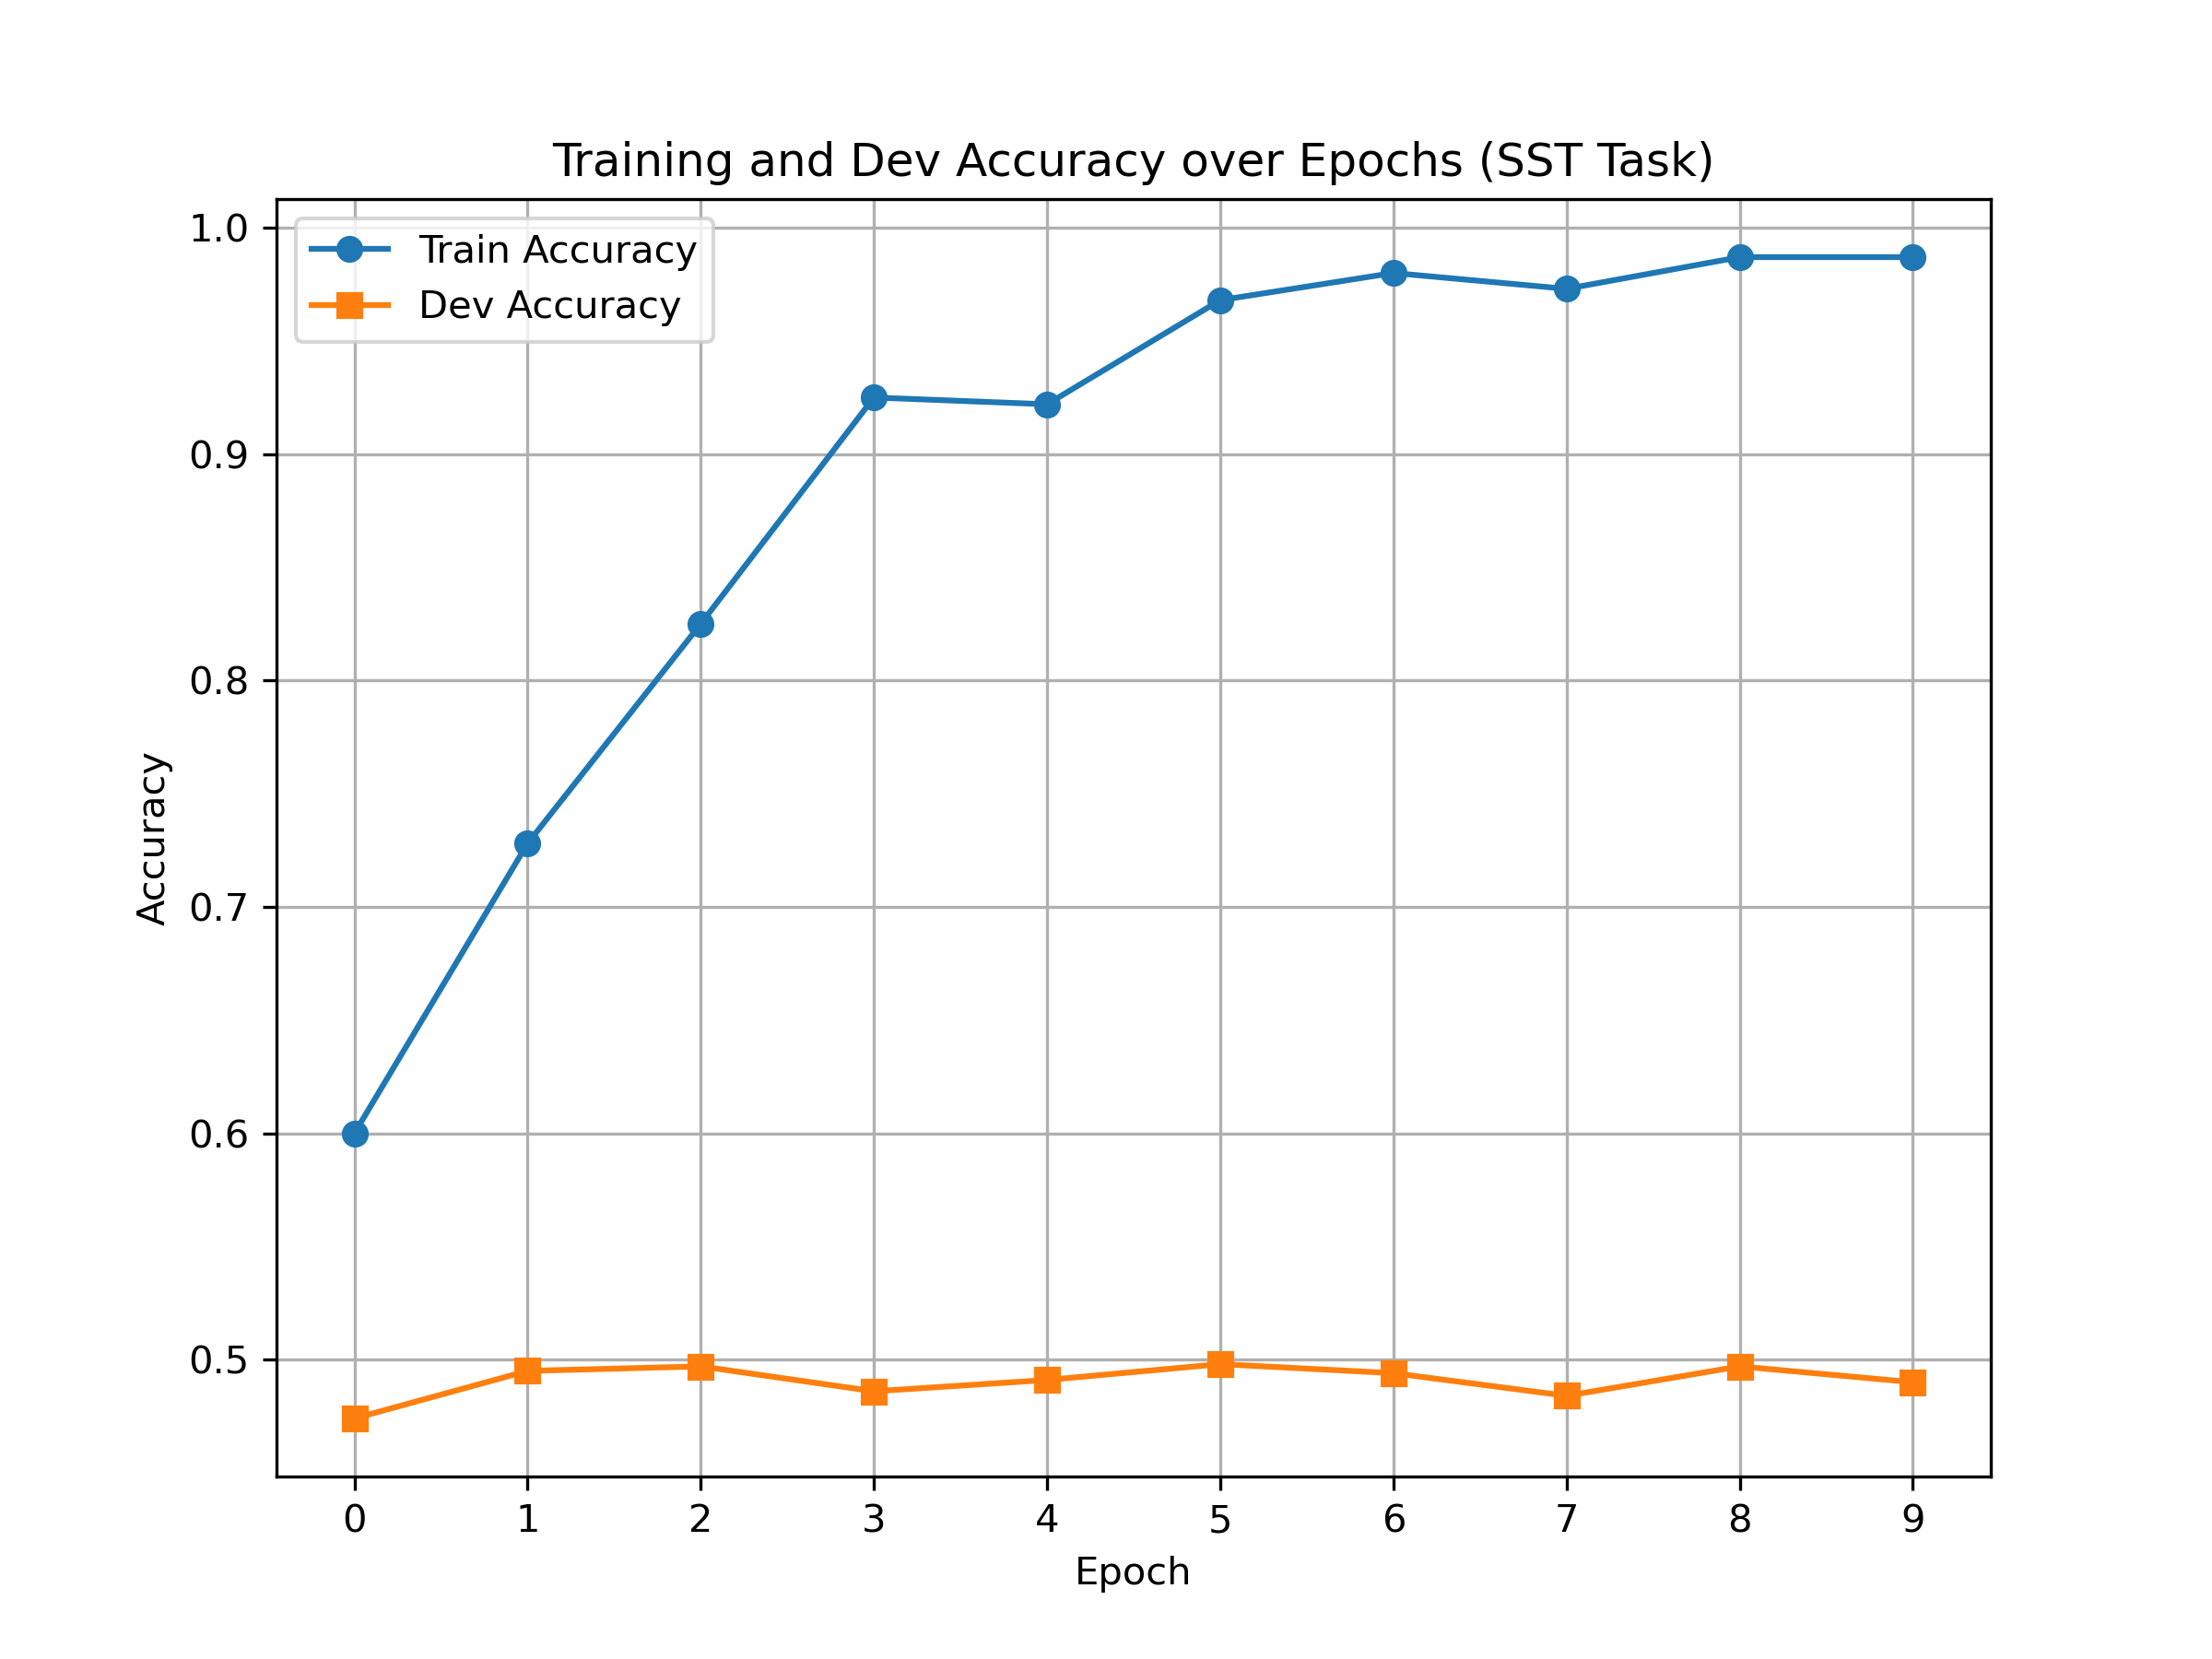
\includegraphics[width=0.7\textwidth]{Figures/SST_plot_10epochs_SBERT_Only.png}
    \caption{Train vs Dev Accuracy for Sentiment Analysis using SBERT Only (10 epochs)}
    \label{fig:sst_acc_plot}
\end{figure}

\begin{table}[H]
    \centering
    \begin{tabular}{|l|l|c|}
    \hline
    \textbf{Task} & \textbf{Metric} & \textbf{Value} \\ \hline
    Paraphrase Detection & Accuracy & 0.7940 \\ \hline
    Semantic Textual Similarity (STS) & Pearson Correlation & 0.6220 \\ \hline
    Sentiment Analysis (SST) & Accuracy & 0.4980 \\ \hline
    \end{tabular}
    \caption{Development set performance after fine-tuning for 10 epochs on SST}
    \label{tab:post_finetuning_metrics}
\end{table}

\begin{itemize}
    \item \textbf{Observations:}
    We observed that training on each task could negatively impact the performance on dissimilar tasks. For example, training on the SST task hurt the model's performance on the STS task. In contrast, training on a particular task improved performance on related tasks. For instance, fine-tuning the model for paraphrase detection improved the correlation score on the STS task, while training on the STS task enhanced the accuracy on the paraphrase detection task.
\end{itemize}

\subsubsection{Sequential Fine-Tuning: SBERT+SMART}
For this training paradigm, we were constrained to use a batch size of 8 due to CUDA out-of-memory errors for higher batch sizes. The SMART regularization technique significantly slowed down training. Specifically, the paraphrase detection task failed for batch sizes above 8. Hence, we decided to use a uniform batch size of 8 across all tasks.

Fine-tuning for paraphrase detection (QQP) took approximately 5 hours per epoch. Due to limited computational resources, we fine-tuned for only one epoch. The development accuracy obtained after this epoch was 0.807. The resulting metrics for all three tasks are summarized in Table~\ref{tab:post_finetuning_metrics_SS}.

\begin{table}[H]
    \centering
    \begin{tabular}{|l|l|c|}
    \hline
    \textbf{Task} & \textbf{Metric} & \textbf{Value} \\ \hline
    Paraphrase Detection & Accuracy & 0.8067 \\ \hline
    Semantic Textual Similarity (STS) & Pearson Correlation & 0.7567 \\ \hline
    Sentiment Analysis (SST) & Accuracy & 0.2089 \\ \hline
    \end{tabular}
    \caption{Development set performance after fine-tuning on Paraphrase Detection for 1 epoch}
    \label{tab:post_finetuning_metrics_SS}
\end{table}

Subsequently, we fine-tuned the model on the STS dataset for 10 epochs. Interestingly, we observed that the highest Pearson correlation was achieved in the first epoch, followed by a consistent decline. This trend is shown in Figure~\ref{fig:SS_sts_corr}.

\begin{figure}[H]
    \centering
    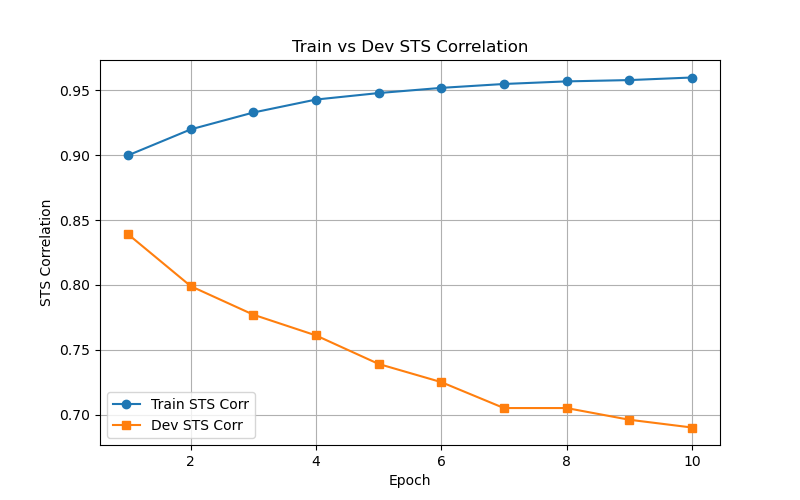
\includegraphics[width=0.7\textwidth]{Figures/SS_sts_corr.png}
    \caption{Train vs Dev Pearson Correlation for STS using SMART SBERT (10 epochs)}
    \label{fig:SS_sts_corr}
\end{figure}

The post-training metrics for all tasks are listed below.

\begin{table}[H]
    \centering
    \begin{tabular}{|l|l|c|}
    \hline
    \textbf{Task} & \textbf{Metric} & \textbf{Value} \\ \hline
    Paraphrase Detection & Accuracy & 0.8045 \\ \hline
    Semantic Textual Similarity (STS) & Pearson Correlation & 0.8394 \\ \hline
    Sentiment Analysis (SST) & Accuracy & 0.2044 \\ \hline
    \end{tabular}
    \caption{Development set performance after fine-tuning for 10 epochs on STS}
    \label{tab:post_finetuning_metrics_SS2}
\end{table}

Finally, we fine-tuned the best model from the STS stage on the SST dataset for 10 epochs. The train vs. dev accuracy trends are illustrated in Figure~\ref{fig:SS_sst_acc}.

\begin{figure}[H]
    \centering
    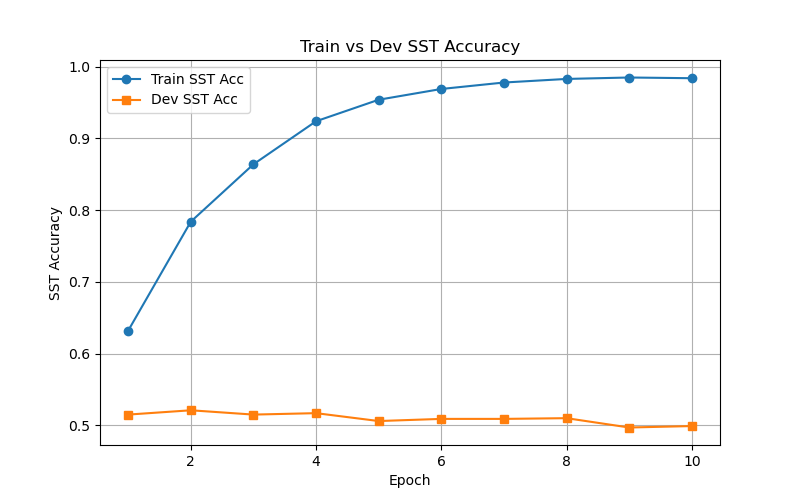
\includegraphics[width=0.7\textwidth]{Figures/SS_sst_acc.png}
    \caption{Train vs Dev Accuracy for SST using SMART SBERT (10 epochs)}
    \label{fig:SS_sst_acc}
\end{figure}

The resulting performance metrics are reported in Table~\ref{tab:post_finetuning_metrics_SS3}.

\begin{table}[H]
    \centering
    \begin{tabular}{|l|l|c|}
    \hline
    \textbf{Task} & \textbf{Metric} & \textbf{Value} \\ \hline
    Paraphrase Detection & Accuracy & 0.7350 \\ \hline
    Semantic Textual Similarity (STS) & Pearson Correlation & 0.7880 \\ \hline
    Sentiment Analysis (SST) & Accuracy & 0.5210 \\ \hline
    \end{tabular}
    \caption{Development set performance after fine-tuning for 10 epochs on SST}
    \label{tab:post_finetuning_metrics_SS3}
\end{table}
We changed the dropout to 0.1 and found that after training for 1 epoch on the paraphrase detection task, the accuracy reached 0.8749. However, when we trained this model on the STS task, the accuracy for STS rose to 0.8580, but the paraphrase detection accuracy dropped to 0.7523. This was due to catastrophic forgetting. Therefore, we decided to train the model as follows:

\begin{enumerate}
    \item Train the model for one epoch on the paraphrase task using the complete dataset.
    \item Train the model for one epoch on the STS dataset (full dataset).
    \item Train the model for one epoch on the SST dataset (full dataset).
    \item Train the model on the paraphrase task using only 3\% of the dataset.
\end{enumerate}

We repeat steps 2 to 4 ten times and save the best model. Overall performance is calculated after training on each task using the following formula:
\[
\text{Overall performance} = \frac{\left( \frac{\text{dev\_sts\_corr} + 1}{2} + \text{sst\_dev\_acc} + \text{paraphrase\_dev\_acc} \right)}{3}
\]

This updated training procedure can be seen in Figure~\ref{fig:Training_Procedure}.

\begin{figure}[H]
    \centering
    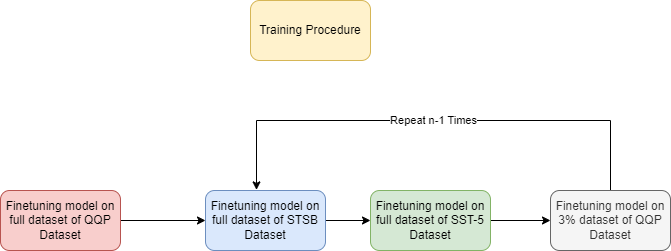
\includegraphics[width=0.7\textwidth]{Figures/Training_Procedure.png}
    \caption{Updated Training Procedure}
    \label{fig:Training_Procedure}
\end{figure}


The optimal model is the one with the highest overall performance across all tasks.

The following table shows the metrics for our best model so far:

\begin{table}[H]
    \centering
    \begin{tabular}{|l|l|c|}
    \hline
    \textbf{Task} & \textbf{Metric} & \textbf{Score} \\
    \hline
    Sentiment Classification & Accuracy & 0.537 \\
    & F1 Score & 0.528 \\
    \hline
    Paraphrase Detection & Accuracy & 0.864 \\
    & F1 Score & 0.864 \\
    \hline
    Semantic Textual Similarity & Pearson Correlation & 0.819 \\
    \hline
    \end{tabular}
    \caption{Evaluation metrics for each task (SMART+SBERT)}
\end{table}
    
Since we changed the training procedure and dropout (from 0.3 to 0.1), it seems logical to retrain the \texttt{SBERT\_Only} model using the new procedure and dropout for a fair comparison.\\
We obtain the following results:

\begin{table}[H]
    \centering
    \begin{tabular}{|l|l|c|}
    \hline
    \textbf{Task} & \textbf{Metric} & \textbf{Score} \\
    \hline
    Sentiment Classification & Accuracy & 0.501 \\
    & F1 Score & 0.495 \\
    \hline
    Paraphrase Detection & Accuracy & 0.854 \\
    & F1 Score & 0.856 \\
    \hline
    Semantic Textual Similarity & Pearson Correlation & 0.680 \\
    \hline
    \end{tabular}
    \caption{Evaluation metrics for each task (SBERT Only)}
\end{table}

\subsubsection{Sequentual Fine-Tuning: SBERT+SimCSE+SMART}
Before applying the training procedure shown in Figure~\ref{fig:Training_Procedure}, we performed contrastive loss minimization (Supervised SimCSE Loss) on the SNLI dataset for 3 epochs, as recommended in \textit{SimCSE: Simple Contrastive Learning of Sentence Embeddings} by Gao et al.~\cite{gao2021simcse}. The best model was selected based on the highest Pearson correlation on the STS-B task. Sentence embeddings were computed as the mean of the token embeddings from the last layer of BERT.
We obtain the following results after this step:
\begin{table}[H]
\centering
\begin{tabular}{|l|l|c|}
\hline
\textbf{Task} & \textbf{Metric} & \textbf{Score} \\
\hline
Sentiment Classification & Accuracy & 0.221 \\
& F1 Score & 0.174 \\
\hline
Paraphrase Detection & Accuracy & 0.626 \\
& F1 Score & 0.503 \\
\hline
Semantic Textual Similarity & Pearson Correlation & 0.812 \\
\hline
\end{tabular}
\caption{Evaluation metrics for each task}
\end{table}

Then after this we begin the training procedure of Figure~\ref{fig:Training_Procedure}. When we train the model for 1 complete QQP datset we get an accuracy of 0.876. However, with the later training we could reach a maximum performance of 0.764. This is lower than what we got for SMART SBERT (Our best model so far).
The results are shown in the table below.

\begin{table}[H]
\centering
\begin{tabular}{|l|l|c|}
\hline
\textbf{Task} & \textbf{Metric} & \textbf{Score} \\
\hline
Sentiment Classification & Accuracy & 0.507 \\
& F1 Score & 0.494 \\
\hline
Paraphrase Detection & Accuracy & 0.864 \\
& F1 Score & 0.863 \\
\hline
Semantic Textual Similarity & Pearson Correlation & 0.843 \\
\hline
\multicolumn{2}{|l|}{\textbf{Overall Performance}} & 0.764 \\
\hline
\end{tabular}
\caption{Evaluation metrics for each task}
\end{table}

\section{Analysis of the Results}
Our best-performing model achieved an overall score of 0.770\%. These results are in line with the top-performing individual models (developed by us) discussed in Section~\ref{subsec:Individually fine-tuned BERT models}. Additionally, our outcomes are competitive with state-of-the-art results reported for each task. The benchmark scores listed in Table~\ref{tab:bert-sota-clean} are sourced from \textit{Papers with Code}~\cite{paperswithcode}.

\begin{table}[H]
\centering
\begin{tabular}{|l|l|c|}
\hline
\textbf{Task} & \textbf{Metric} & \textbf{Score} \\
\hline
Sentiment Classification & Accuracy & 0.532 \\
\hline
Paraphrase Detection & Accuracy & 0.910 \\
\hline
Semantic Textual Similarity & Pearson Correlation & 0.8479 \\
\hline
\multicolumn{2}{|l|}{\textbf{Overall Performance}} & 0.7887 \\
\hline
\end{tabular}
\caption{State-of-the-art BERT-base results for each task}
\label{tab:bert-sota-clean}
\end{table}

We have two strong models: SMART SBERT (SS) and SMART SBERT with SimCSE (SSS). Both SS and SSS perform approximately equally well on the paraphrase detection task. However, SS performs better on the SST-5 task, while SSS performs better on the STS-B task. The superior performance of SSS on STS-B is understandable, as the supervised SimCSE loss is specifically optimized to enhance performance on semantic textual similarity tasks such as STS-B. Depending on the task priority, either of the two models can be selected.